\chapter{Implementierung}
\label{chapter:Implementierung}




%%%%%%%%%%%%%%%%%%%%%%%%%%%%%%%%%%%%%%%%%%%%%%%%%%%%%%%%%%%%%%%%%%%%%%%%%%%%%%%%%%%%
%%%%%%%%%%%%%%%%%%%%%%%%%%%%%%%%%%%%%%%%%%%%%%%%%%%%%%%%%%%%%%%%%%%%%%%%%%%%%%%%%%%%
%%%%%%%%%%%%%%%%%%%%%%%%%%%%%%%%%%%%%%%%%%%%%%%%%%%%%%%%%%%%%%%%%%%%%%%%%%%%%%%%%%%%
%%%%%%%%%%%%%%%%%%%%%%%%%%%%%%%%%%%%%%%%%%%%%%%%%%%%%%%%%%%%%%%%%%%%%%%%%%%%%%%%%%%%
%%%%%%%%%%%%%%%%%%%%%%%%%%%%%%%%%%%%%%%%%%%%%%%%%%%%%%%%%%%%%%%%%%%%%%%%%%%%%%%%%%%%
%%%%%%%%%%%%%%%%%%%%%%%%%%%%%%%%%%%%%%%%%%%%%%%%%%%%%%%%%%%%%%%%%%%%%%%%%%%%%%%%%%%%


\section{Auswahl der Bauteile}
\label{section:Auswahl_der_Bauteile}

Für das Projekt wurden die echtzeitfähige Steuerung, die Batterie, der Motor und die zugehörige Steuerung vorgegeben. Alle weiteren Bauteile mussten bestellt werden.




%%%%%%%%%%%%%%%%%%%%%%%%%%%%%%%%%%%%%%%%%%%%%%%%%%%%%%%%%%%%%%%%%%%%%%%%%%%%%%%%%%%%
%%%%%%%%%%%%%%%%%%%%%%%%%%%%%%%%%%%%%%%%%%%%%%%%%%%%%%%%%%%%%%%%%%%%%%%%%%%%%%%%%%%%
%%%%%%%%%%%%%%%%%%%%%%%%%%%%%%%%%%%%%%%%%%%%%%%%%%%%%%%%%%%%%%%%%%%%%%%%%%%%%%%%%%%%
%%%%%%%%%%%%%%%%%%%%%%%%%%%%%%%%%%%%%%%%%%%%%%%%%%%%%%%%%%%%%%%%%%%%%%%%%%%%%%%%%%%%
%%%%%%%%%%%%%%%%%%%%%%%%%%%%%%%%%%%%%%%%%%%%%%%%%%%%%%%%%%%%%%%%%%%%%%%%%%%%%%%%%%%%
%%%%%%%%%%%%%%%%%%%%%%%%%%%%%%%%%%%%%%%%%%%%%%%%%%%%%%%%%%%%%%%%%%%%%%%%%%%%%%%%%%%%


\section{Schaltplan}
\label{section:Schaltplan}


\myboxy{
	\begin{itemize}
		\item Funktion (=Anlage) und Ortskennzeichen (+Ort) definieren. Funktionales Engineering.
		\item Bauteilkennzeichnung (BMK) festlegen.
		\item Aderfarben und Querschnitt definieren.
		\item Ausgewählte Bauteile in die Schaltung integrieren.
		\item Nicht vorhandene Bauteile selbst erstellen.
		      \begin{itemize}
			      \item Bauteile sortiert hinzufügen: Spannungsversorgung, Steuerung (Eingang, dann Ausgang), Lastkreis und Sonderfunktionen.
		      \end{itemize}
	\end{itemize}}{To-do}{\textwidth}



Zu Beginn der Erstellung des Schaltplans sollten die Funktions- und Ortskennzeichen sowie die Beschriftung der Bauteile und Leitungen festgelegt werden. Bei der Verdrahtung ist es erforderlich, die Aderfarben den entsprechenden Spannungspotenzialen zuzuordnen.

\subsection{Betriebsmittelbezeichnung}
\label{Schaltplan:BMK}

Ein Betriebsmittel besteht aus verschiedenen Kennzeichen: dem Funktionskennzeichen (=), dem Ortskennzeichen (+) und dem Betriebsmittelkennzeichen (-). Früher wurde das Funktionskennzeichen als „Anlage“ bezeichnet. In der neuen DIN EN IEC 81346-2 \cite{DIN_EN_IEC_81346-2} wurde diese Bezeichnung jedoch auf „Funktion“ geändert.

\subsubsection{Funktionskennzeichen}
Das Funktionskennzeichen beschreibt eine bestimmte Funktion im Schaltplan, wie beispielsweise die Spannungsversorgung oder die Steuerung (siehe Tabelle \ref{BMK:tab:funktionskennzeichen}).

\pagebreak[1]
\begin{table}[!ht]
	\centering
	\caption{Schaltplan – Funktionskennzeichen (=)}
	\label{BMK:tab:funktionskennzeichen}
	\begin{tabular}{ll}
		\hline
		\textbf{Abkürzung}      & \textbf{Bezeichnung} \\ \hline
		\multicolumn{1}{l|}{SV} & Spannungsversorung   \\
		\multicolumn{1}{l|}{ES} & Eingänge Steuerung   \\
		\multicolumn{1}{l|}{AS} & Ausgänge Steuerung   \\
		\multicolumn{1}{l|}{KO} & Kommunikation        \\
		\multicolumn{1}{l|}{AT} & Antrieb              \\
		\multicolumn{1}{l|}{NA} & Not-Aus              \\ \hline
	\end{tabular}
\end{table}
\pagebreak[1]

\subsubsection{Ortskennzeichen}
Das Ortskennzeichen gibt an, an welchem Ort ein Bauteil installiert ist. Beispielsweise gibt es im Fahrzeug eine Steuereinheit und eine Batterieeinheit. Im Schaltplan wird dadurch deutlich, welche Verbindungen zwischen verschiedenen Orten bestehen. Das Ortskennzeichen erleichtert zudem die Wartung und Installation des Systems.

\pagebreak[1]
\begin{table}[!ht]
	\centering
	\caption{Schaltplan – Ortskennzeichen (+)}
	\label{bmk:tab:ortskennzeichen}
	\begin{tabular}{ll}
		\hline
		\textbf{Abkürzung}       & \textbf{Bezeichnung} \\ \hline
		\multicolumn{1}{l|}{POD} & Fahrzeug             \\
		\multicolumn{1}{l|}{BE}  & Batterieeinheit      \\
		\multicolumn{1}{l|}{SE}  & Steuereinheit        \\
		\multicolumn{1}{l|}{AE}  & Antriebseinheit      \\ \hline
	\end{tabular}
\end{table}
\pagebreak[1]

\subsubsection{Betriebsmittelkennzeichen}
Das Betriebsmittelkennzeichen bezeichnet das spezifische Bauteil. Die genaue Zuordnung der Bezeichnungen ist in der DIN EN IEC 81346-2 geregelt. Die für das Projekt relevanten Betriebsmittelkennzeichen sind in Tabelle \ref{bmk:tab:betriebsmittelkennzeichen} aufgeführt.



\pagebreak[1]
\begin{table}[!ht]
	\centering
	\caption{Schaltplan – Betriebsmittelkennzeichen (-) \cite{DIN_EN_IEC_81346-2}}
	\label{bmk:tab:betriebsmittelkennzeichen}
	\begin{tabular}{|l|lll|}
		\hline
		\textbf{Abkürzung}       & \textbf{Klassenname}                            & \multicolumn{1}{l|}{\textbf{Allgemeine Bedeutung}} \\ \hline
		\multicolumn{1}{|l|}{FC} & \makecell[l]{Überstromschutzobjekt}             & \multicolumn{1}{l|}{Sicherung}                     \\ \hline
		\multicolumn{1}{|l|}{GB} & \makecell[l]{Erzeugungsobjekt für elektrische                                                        \\Energie durch chemische Energie} & \multicolumn{1}{l|}{Batterie} \\ \hline
		\multicolumn{1}{|l|}{KE} & \makecell[l]{Elektrische Signale                                                                     \\verarbeitendes Objekt}   & \multicolumn{1}{l|}{Steuerung} \\ \hline
		\multicolumn{1}{|l|}{MA} & \makecell[l]{Elektromagnetisches                                                                     \\Rotationsantriebsobjekt} & \multicolumn{1}{l|}{Motor} \\ \hline
		\multicolumn{1}{|l|}{QA} & \makecell[l]{Stromsteuerungsobjekt}             & \multicolumn{1}{l|}{Relais}                        \\ \hline
		\multicolumn{1}{|l|}{RL} & \makecell[l]{Bewegungsbegrenzungsobjekt}        & \multicolumn{1}{l|}{Bremse}                        \\ \hline
		\multicolumn{1}{|l|}{SF} & \makecell[l]{Gesichtsinteraktionsobjekt}        & \multicolumn{1}{l|}{Schalter}                      \\ \hline
		\multicolumn{1}{|l|}{TB} & \makecell[l]{Stromkonvertierungsobjekt}         & \multicolumn{1}{l|}{Transformator}                 \\ \hline
		\multicolumn{1}{|l|}{WD} & \makecell[l]{Niederspannungsenergie Leitobjekt} & \multicolumn{1}{l|}{Leitung/Kabel}                 \\ \hline
		\multicolumn{1}{|l|}{XD} & \makecell[l]{Niederspannungs-Verbindungsobjekt} & \multicolumn{1}{l|}{Klemme, Stecker oder Buchse}   \\ \hline
	\end{tabular}
\end{table}
\pagebreak[1]

Bei einer vollständigen Betriebsmittelbezeichnung sieht das Kennzeichen des Betriebsmittels folgendermaßen aus:

\begin{center} =ES2+SE1-10QA1 \end{center}

Die Betriebsmittelbezeichnung =ES2+SE1-10QA4 besagt, dass es sich um die Eingänge der Steuerung (=ES) handelt, wobei es zwei Funktionen gibt. Der Ort ist in der Steuereinheit (+SE) verortet, und das Betriebsmittel selbst ist ein Relais, das auf der Seite 10 des Schaltplans zu finden ist.

Das Kennzeichen umfasst sowohl das Funktions- als auch das Ortskennzeichen, die jeweils mit einer fortlaufenden Nummer versehen sind. Das Betriebsmittelkennzeichen enthält zwei Nummerierungen: Die erste gibt an, auf welcher Seite des Schaltplans sich das Betriebsmittel befindet, während die zweite die fortlaufende Nummerierung des Bauteils darstellt.\\
Im Schaltplan wird das Betriebsmittel lediglich durch das Betriebsmittelkennzeichen (-) dargestellt, während das Funktions- und Ortskennzeichen im Zeichnungskopf angegeben ist.

\newpage

\subsection{Verdrahtung Konventionen}
\label{section:Verdrahtung_Konventionen}
Für die Verdrahtung müssen den Spannungspotenzialen verschiedene Farben zugewiesen werden. Diese Zuordnungen sind in Tabelle \ref{Verdrahtung_Konventionen:tab:Zuordnung} aufgeführt.
\pagebreak[1]
\begin{table}[ht!]
	\centering
	\caption{Verdrahtung Konvention – Aderfarben}
	\label{Verdrahtung_Konventionen:tab:Zuordnung}
	\begin{tabular}{llccl}
		\hline
		\textbf{Name} & \textbf{Fabe}                 & \textbf{U in V} & \textbf{A in mm$^2$} & \textbf{Funktion} \\ \hline
		              & \multicolumn{1}{l|}{Rot}      & $x$             & 1                    &                   \\
		              & \multicolumn{1}{l|}{Blau}     & $x$             & 1                    &                   \\
		              & \multicolumn{1}{l|}{Schwarz}  & $x$             & 1                    &                   \\
		              & \multicolumn{1}{l|}{Schwarz}  & $< 48$          & 50                   &                   \\
		              & \multicolumn{1}{l|}{Viollett} & $x$             & 1                    &                   \\ \hline
	\end{tabular}
\end{table}
\pagebreak[4]




%%%%%%%%%%%%%%%%%%%%%%%%%%%%%%%%%%%%%%%%%%%%%%%%%%%%%%%%%%%%%%%%%%%%%%%%%%%%%%%%%%%%
%%%%%%%%%%%%%%%%%%%%%%%%%%%%%%%%%%%%%%%%%%%%%%%%%%%%%%%%%%%%%%%%%%%%%%%%%%%%%%%%%%%%
%%%%%%%%%%%%%%%%%%%%%%%%%%%%%%%%%%%%%%%%%%%%%%%%%%%%%%%%%%%%%%%%%%%%%%%%%%%%%%%%%%%%
%%%%%%%%%%%%%%%%%%%%%%%%%%%%%%%%%%%%%%%%%%%%%%%%%%%%%%%%%%%%%%%%%%%%%%%%%%%%%%%%%%%%
%%%%%%%%%%%%%%%%%%%%%%%%%%%%%%%%%%%%%%%%%%%%%%%%%%%%%%%%%%%%%%%%%%%%%%%%%%%%%%%%%%%%
%%%%%%%%%%%%%%%%%%%%%%%%%%%%%%%%%%%%%%%%%%%%%%%%%%%%%%%%%%%%%%%%%%%%%%%%%%%%%%%%%%%%

\newpage
\section{Simulation mit Simulink}
\label{section:Simulation}

\myboxy{
	\begin{itemize}
		\item
	\end{itemize}
}{To-do}{\textwidth}


\subsection{Funktionsweise der Steuerung}
\label{Steuerung}

%Das Fahrzeug wird mittels eines Moore-Automaten gesteuert, wie in Abbildung \ref{Automat:img:Automat} dargestellt. Die Zustände $\overrightarrow{Z}$ (siehe Gleichung \ref{Automat:equation:vektor_z_auto}), die Eingänge $\overrightarrow{I}$ (siehe Gleichung \ref{Automat:equation:vektor_i}) und die Ausgänge $\overrightarrow{O}$ (siehe Gleichung \ref{Automat:equation:vektor_o}) können in Vektoren dargestellt werden.\\ \ \\

Die Steuerung des Fahrzeugs bietet die Möglichkeit, zwischen Automatik- und manuellem Betrieb zu wählen. Im manuellen Betrieb kann der Benutzer das Fahrzeug sowohl vorwärts als auch rückwärts fahren lassen, wobei zwei Geschwindigkeitsstufen – schnell und langsam – zur Verfügung stehen.\\
Der Automatikmodus wird über den Startknopf aktiviert. Das Fahrzeug beschleunigt auf die einstellbare Geschwindigkeit und bremst automatisch ab, sobald die Distanz zum Enddeckel der Röhre kleiner wird. Es hält schließlich am Ende der Strecke an.\\

\subsubsection{Controllpanel}
\label{Steuerung:Controllpanel}
Über das Control Panel (siehe Abbildung \ref{Controllpanel:img:Controllpanel}) können alle Eingaben via Simulink gesteuert werden, welche im Folgenden erklärt werden. Mit dem Wahlschalter kann zwischen Automatik- und manuellem Betrieb gewechselt werden. Ist der manuelle Betrieb ausgewählt, kann mit dem Drehschalter (Manuell) zwischen Vorwärts, Rückwärts und Stopp geschaltet werden (siehe Tabelle \ref{Controllpanel:tab:Wahlschalter}, die Werte werden später für die Automaten Steuerung benötigt).\\


\pagebreak[1]
\begin{table}[!ht]
	\centering
	\caption{Automat – Wahlschalter für den manuellen Betrieb}
	\label{Controllpanel:tab:Wahlschalter}
	\begin{tabular}{cll}
		\hline
		\textbf{Schalterbezeichnung} & \textbf{Zustand} & \textbf{Wert} \\ \hline
		\multicolumn{1}{l|}{Rück+}   & V schnell        & 1             \\
		\multicolumn{1}{l|}{Rück}    & R langsam        & 2             \\
		\multicolumn{1}{l|}{STOP}    & Manuell idle     & 3             \\
		\multicolumn{1}{l|}{Vor}     & V langsam        & 4             \\
		\multicolumn{1}{l|}{Vor+}    & V schnell        & 5             \\ \hline
	\end{tabular}
\end{table}
\pagebreak[3]
Im Automatikbetrieb kann die Geschwindigkeit über das Drehrad \frqq Geschwindigkeit Automatik\flqq\ voreingestellt oder während der Fahrt angepasst werden. Das Fahrzeug beginnt zu fahren, sobald der Druckknopf \frqq Start\flqq\ betätigt wird. Die Automatik kann über den Druckknopf \frqq Stop\flqq\ gestoppt werden.\\ Im Notfall kann sowohl im Automatik- als auch im manuellen Betrieb der Druckknopf \frqq Emergency stop\flqq\ betätigt werden. Das Fahrzeug führt eine Vollbremsung mit der Motor- und der mechanischen Bremse durch. Der Notfallmodus kann durch Drücken des \frqq Reset\flqq\ -Knopfs beendet werden.\\
Die Funktionsweise der manuellen Steuerung wird in Abschnitt \ref{Automatensteuerung:Automat_man} erklärt, und die der automatischen Steuerung in Abschnitt \ref{Automatensteuerung:Automat_auto}


\pagebreak[1]
\begin{figure}[!ht]
	\begin{center}
		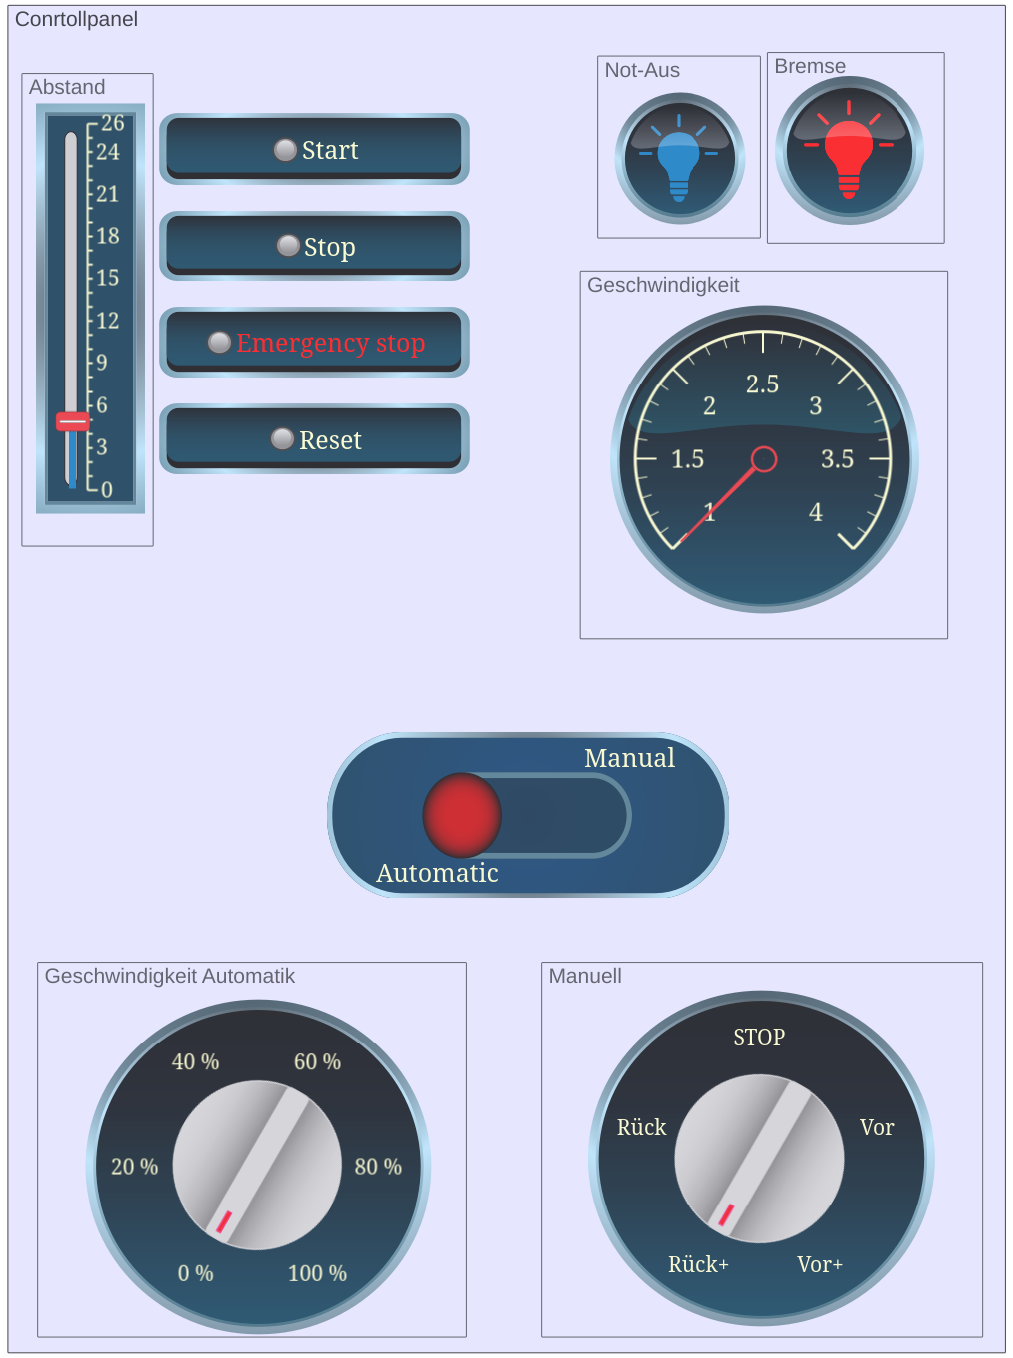
\includegraphics[width=0.75\textwidth]{img/5_simulation/Automat_con.png}
		\caption{Automat – Controllpanel}
		\label{Controllpanel:img:Controllpanel}
	\end{center}
\end{figure}
\pagebreak[4]


\subsection{Automatensteuerung}
\label{Automatensteuerung}
Die Automatensteuerung beschreibt die logische Steuerung eines Systems durch einen Automaten, wie etwa einen Moore- oder Mealy-Automaten, der auf Basis von Eingaben und aktuellen Zuständen Ausgaben steuert.\\
Das Fahrzeug wird mittels eines Moore-Automaten gesteuert, wobei die Ausgänge erst dann aktiviert werden, wenn sich das System im entsprechenden Zustand befindet.\\ \ \\
Der Automat startet im Zustand \frqq IDLE\flqq, und die Abläufe für den automatischen oder manuellen Modus werden von \frqq IDLE\flqq\ aus angesteuert. Im Zustand Idle werden die Ausgänge (siehe Tabelle \ref{Automat_man:tab:z_idle}) geschaltet.\\


\pagebreak[1]
\begin{table}[!ht]
	\centering
	\caption{Ausgänge – Idle}
	\label{Automat_man:tab:z_idle}
	\begin{tabular}{lll}
		\hline
		\textbf{Ausgänge}                           & \textbf{I/O Module}                 & \textbf{Wert} \\ \hline
		\multicolumn{1}{l|}{speed out}              & \multicolumn{1}{l|}{IO397-50k – A1} & 1             \\
		\multicolumn{1}{l|}{Driving(1)}             & \multicolumn{1}{l|}{}               & Reset         \\
		\multicolumn{1}{l|}{break motor out}        & \multicolumn{1}{l|}{IO397-50k – B3} & 5             \\
		\multicolumn{1}{l|}{direction out}          & \multicolumn{1}{l|}{IO397-50k – B4} & 5             \\
		\multicolumn{1}{l|}{cruise out}             & \multicolumn{1}{l|}{IO397-50k – B5} & 5             \\
		\multicolumn{1}{l|}{break mechanically out} & \multicolumn{1}{l|}{IO397-50k – B6} & 5             \\
		\multicolumn{1}{l|}{emergency stop out}     & \multicolumn{1}{l|}{IO397-50k – B7} & 0             \\ \hline
	\end{tabular}
\end{table}
\pagebreak[1]

Die Funktion Driving, siehe Abbildung \ref{Automat:img:fnc_Driving}, erhält einen Eingangswert, der durch einen \frqq Rate Limiter\flqq\ begrenzt und am Ausgang ausgegeben wird. Die Funktion speichert den letzten Wert, daher muss sie in den Zuständen, in denen das Fahrzeug angehalten wird, zurückgesetzt werden. Dies geschieht, indem die Funktion Driving den Wert 1 erhält.\\

\pagebreak[1]
\begin{figure}[!ht]
	\begin{center}
		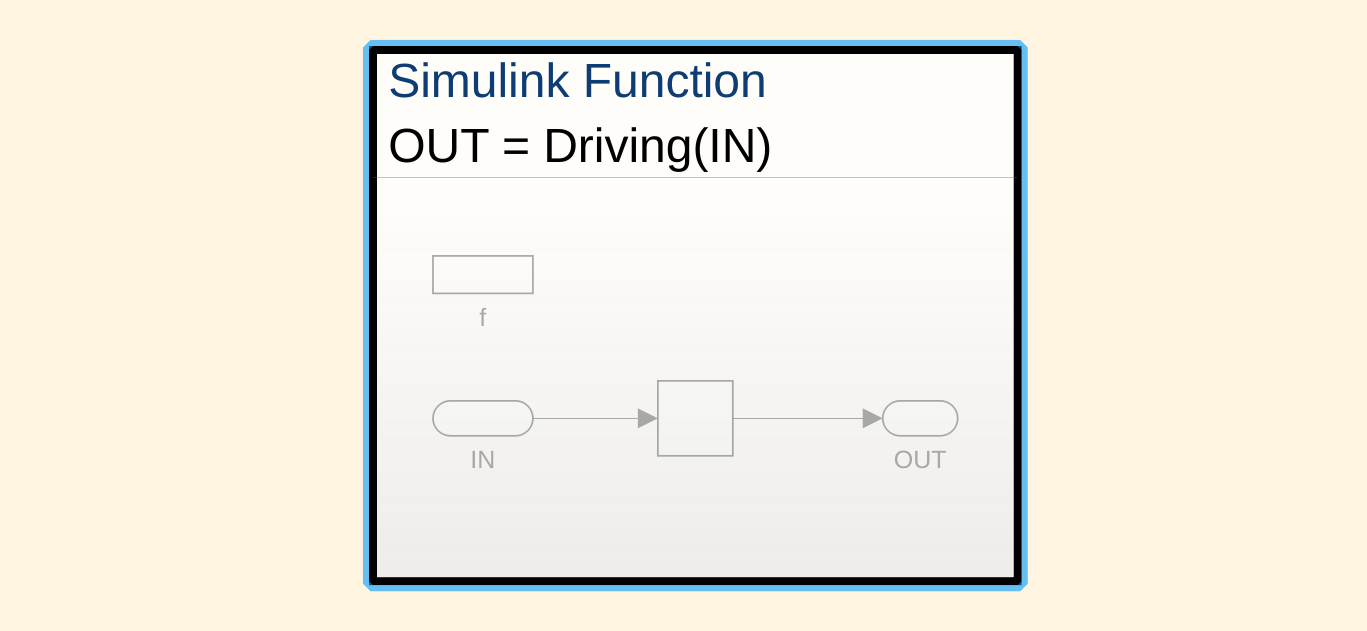
\includegraphics[width=.5\textwidth]{img/5_simulation/Automat_funktion_1.png}
		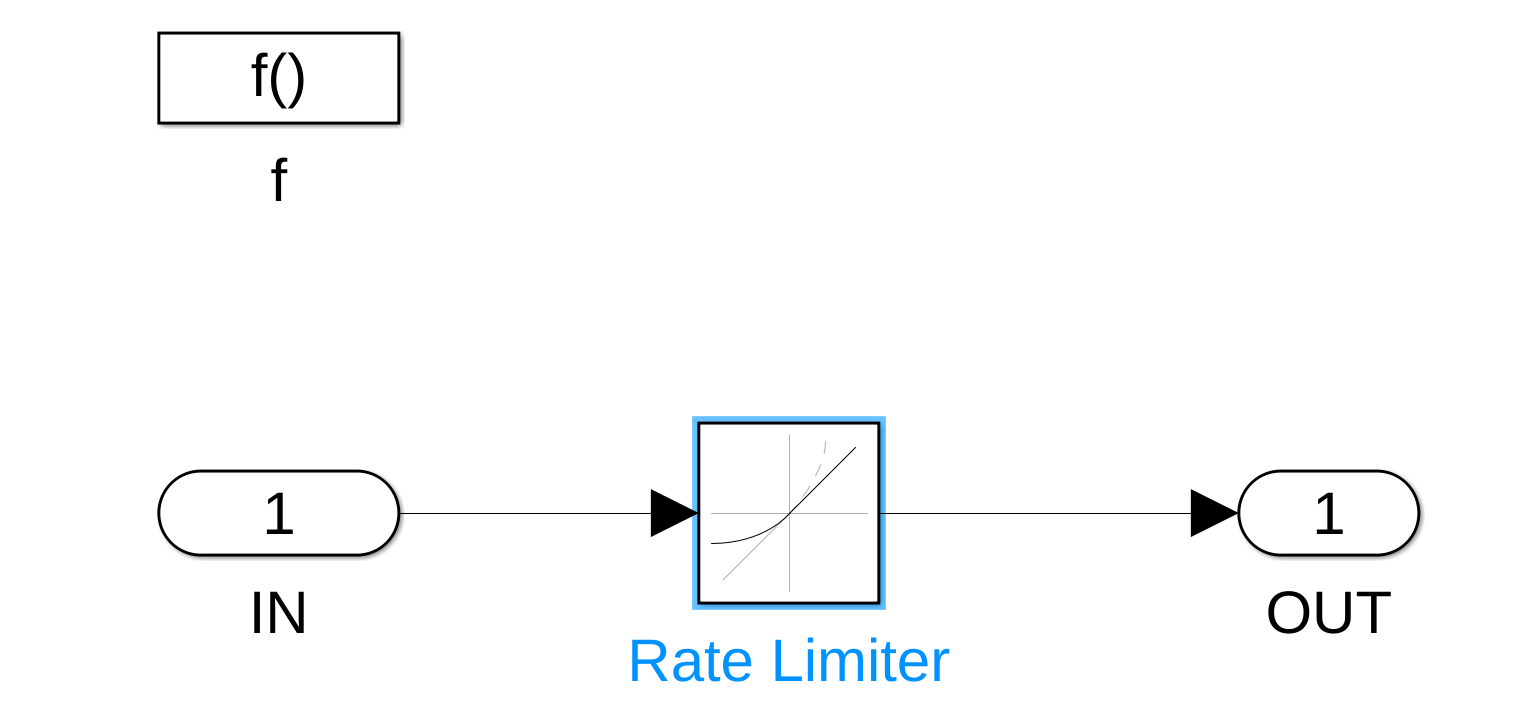
\includegraphics[width=.75\textwidth]{img/5_simulation/Automat_funktion_2.png}
		\caption{Automat – Funktion Driving}
		\label{Automat:img:fnc_Driving}
	\end{center}
\end{figure}
\pagebreak[4]

Zustand \frqq Emergency stop\flqq\ kann von jedem Zustand aus durch den Eingang \frqq emergency stop in\flqq\ erreicht werden, welcher sowohl über das Controllpanel als auch extern über das IO397-50k – B11 ausgelöst werden kann. Der Zustand kann nur durch ein Reset-Signal verlassen werden und führt dann in einen der Idle-Zustände zurück: Idle, manuell idle oder automatik idle zurück. Im Zustand \frqq Emergency stop\flqq\ werden die Ausgänge gemäß Tabelle \ref{Automat_man:tab:z_Emergency_stop} geschaltet.


\pagebreak[1]
\begin{table}[!ht]
	\centering
	\caption{Ausgänge – Emergency stop}
	\label{Automat_man:tab:z_Emergency_stop}
	\begin{tabular}{lll}
		\hline
		\textbf{Ausgänge}                           & \textbf{I/O Module}                 & \textbf{Wert} \\ \hline
		\multicolumn{1}{l|}{speed out}              & \multicolumn{1}{l|}{IO397-50k – A1} & 1             \\
		\multicolumn{1}{l|}{Driving(1)}             & \multicolumn{1}{l|}{}               & Reset         \\
		\multicolumn{1}{l|}{break motor out}        & \multicolumn{1}{l|}{IO397-50k – B3} & 5             \\
		\multicolumn{1}{l|}{direction out}          & \multicolumn{1}{l|}{IO397-50k – B4} & 5             \\
		\multicolumn{1}{l|}{cruise out}             & \multicolumn{1}{l|}{IO397-50k – B5} & 5             \\
		\multicolumn{1}{l|}{break mechanically out} & \multicolumn{1}{l|}{IO397-50k – B6} & 5             \\
		\multicolumn{1}{l|}{emergency stop out}     & \multicolumn{1}{l|}{IO397-50k – B7} & 5             \\ \hline
	\end{tabular}
\end{table}
\pagebreak[4]

%\pagebreak[1]
%\begin{figure}[!ht]
%	\begin{center}
%		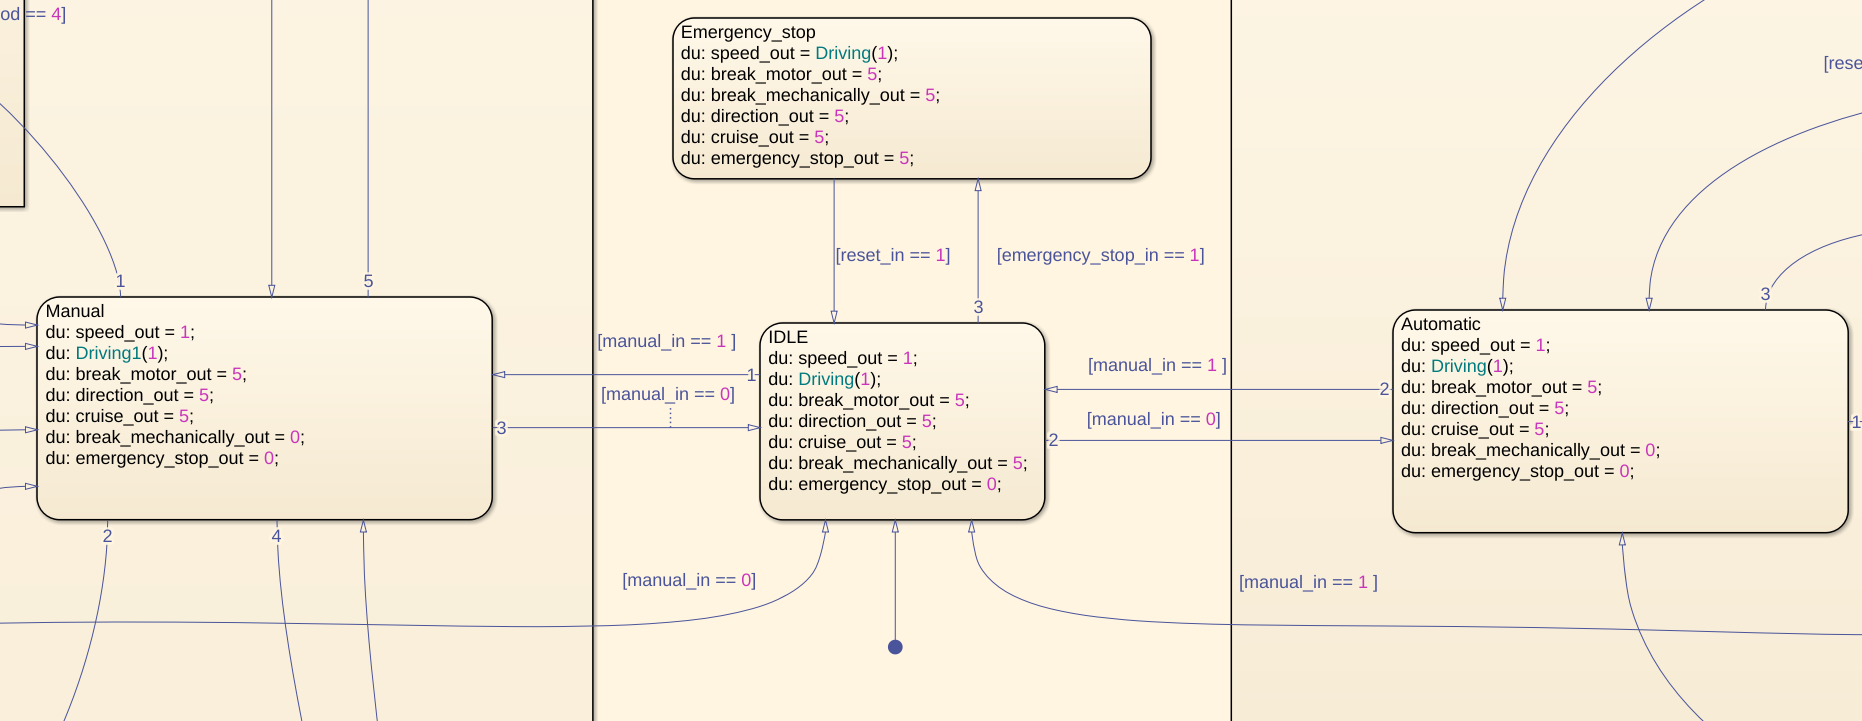
\includegraphics[width=\textwidth]{img/5_simulation/Automat_idle.png}
%		\caption{Automat – Start Zustand \frqq IDLE\flqq}
%		\label{Automat_man:img:start_idle}
%	\end{center}
%\end{figure}
%\pagebreak[4]








\subsubsection{Automat für die manuelle Steuerung}
\label{Automatensteuerung:Automat_man}

Der Automat des manuellen Ablaufs, wie in Abbildung \ref{Automat_man:img:man_übersicht} dargestellt, ist in zwei Stateflows unterteilt: \frqq vorwärts\flqq\ und \frqq rückwärts\flqq . In Abbildung \ref{Automat_man:img:man_vorwärts} ist der \frqq vorwärts\flqq\ -Stateflow zu sehen, der \frqq rückwärts\flqq\ -Stateflow ist äquivalent, wobei sich lediglich der Ausgang \frqq Direction Out\flqq\ ändert. Daher wird nur der \frqq vorwärts\flqq\ -Stateflow erklärt. Die Ausgänge für die Zustände \frqq vorwärts\flqq\ und \frqq rückwärts\flqq\ sind in der Tabelle \ref{Automat_man:tab:z_V_langsam} für die Zustände \frqq langsam\flqq\ und in der Tabelle \ref{Automat_man:tab:z_V_schnell} für die Zustände \frqq schnell\flqq\ aufgelistet.




\pagebreak[1]
\begin{figure}[!ht]
	\begin{center}
		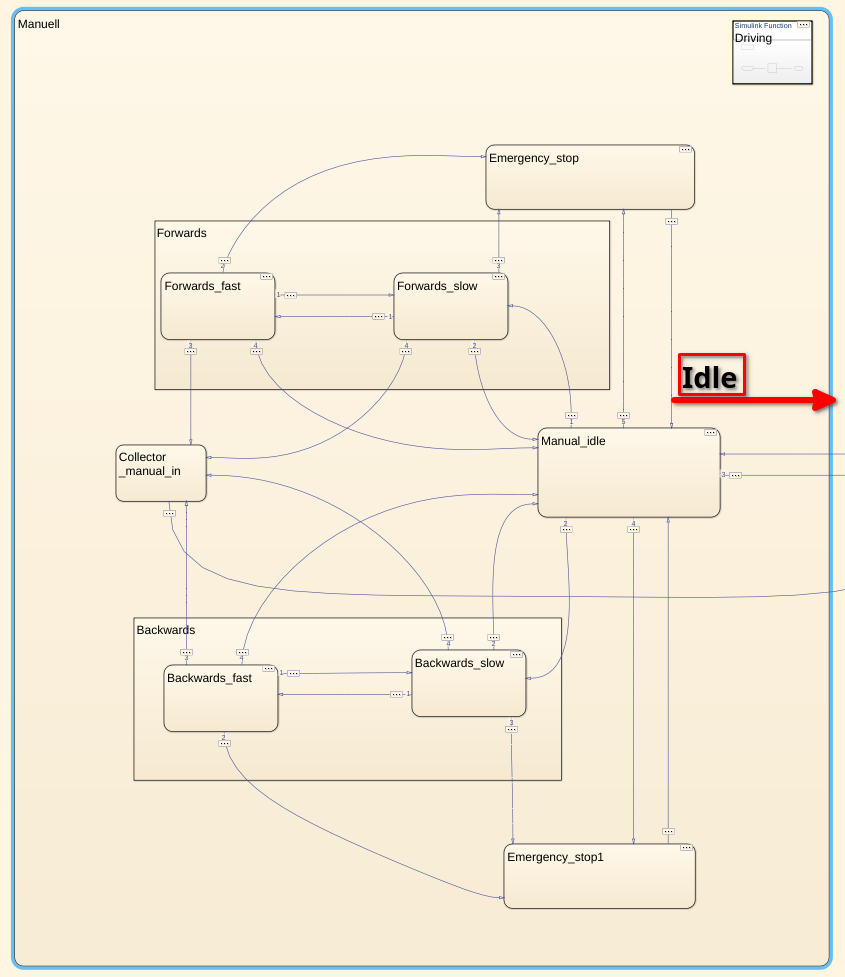
\includegraphics[width=0.9\textwidth]{img/5_simulation/Automat_man_uebersicht.png}
		\caption{Automat – Übersicht der manuellen Steuerung}
		\label{Automat_man:img:man_übersicht}
	\end{center}
\end{figure}
\pagebreak[1]


\pagebreak[1]
\begin{table}[!ht]
	\centering
	\caption{Ausgänge – der Zustände vorwärts und rückwärts langsam}
	\label{Automat_man:tab:z_V_langsam}
	\begin{tabular}{llcc}
		\hline
		\textbf{Ausgänge}                               & \textbf{I/O Module}                 & \makecell{\textbf{Werte}     \\ \textbf{Vorwärts}} & \makecell{\textbf{Werte}     \\ \textbf{Rückwärts}}  \\ \hline
		\multicolumn{1}{l|}{speed out = Driving$(1,5)$} & \multicolumn{1}{l|}{IO397-50k – A1} & 1,5                      & 3 \\
		\multicolumn{1}{l|}{break motor out}            & \multicolumn{1}{l|}{IO397-50k – B3} & 1                        & 1 \\
		\multicolumn{1}{l|}{direction out}              & \multicolumn{1}{l|}{IO397-50k – B4} & 5                        & 0 \\
		\multicolumn{1}{l|}{cruise out}                 & \multicolumn{1}{l|}{IO397-50k – B5} & 5                        & 5 \\
		\multicolumn{1}{l|}{break mechanically out}     & \multicolumn{1}{l|}{IO397-50k – B6} & 0                        & 0 \\
		\multicolumn{1}{l|}{emergency stop out}         & \multicolumn{1}{l|}{IO397-50k – B7} & 0                        & 0 \\ \hline
	\end{tabular}
\end{table}
\pagebreak[1]

\pagebreak[1]
\begin{table}[!ht]
	\centering
	\caption{Ausgänge – der Zustände vorwärts und rückwärts schnell}
	\label{Automat_man:tab:z_V_schnell}
	\begin{tabular}{llcc}
		\hline
		\textbf{Ausgänge}                             & \textbf{I/O Module}                 & \makecell{\textbf{Werte}     \\ \textbf{Vorwärts}} & \makecell{\textbf{Werte}     \\ \textbf{Rückwärts}} \\ \hline
		\multicolumn{1}{l|}{speed out = Driving$(3)$} & \multicolumn{1}{l|}{IO397-50k – A1} & 3                        & 3 \\
		\multicolumn{1}{l|}{break motor out}          & \multicolumn{1}{l|}{IO397-50k – B3} & 1                        & 1 \\
		\multicolumn{1}{l|}{direction out}            & \multicolumn{1}{l|}{IO397-50k – B4} & 5                        & 0 \\
		\multicolumn{1}{l|}{cruise out}               & \multicolumn{1}{l|}{IO397-50k – B5} & 5                        & 5 \\
		\multicolumn{1}{l|}{break mechanically out}   & \multicolumn{1}{l|}{IO397-50k – B6} & 0                        & 0 \\
		\multicolumn{1}{l|}{emergency stop out}       & \multicolumn{1}{l|}{IO397-50k – B7} & 0                        & 0 \\ \hline
	\end{tabular}
\end{table}
\pagebreak[1]

\pagebreak[1]
\begin{figure}[!ht]
	\begin{center}
		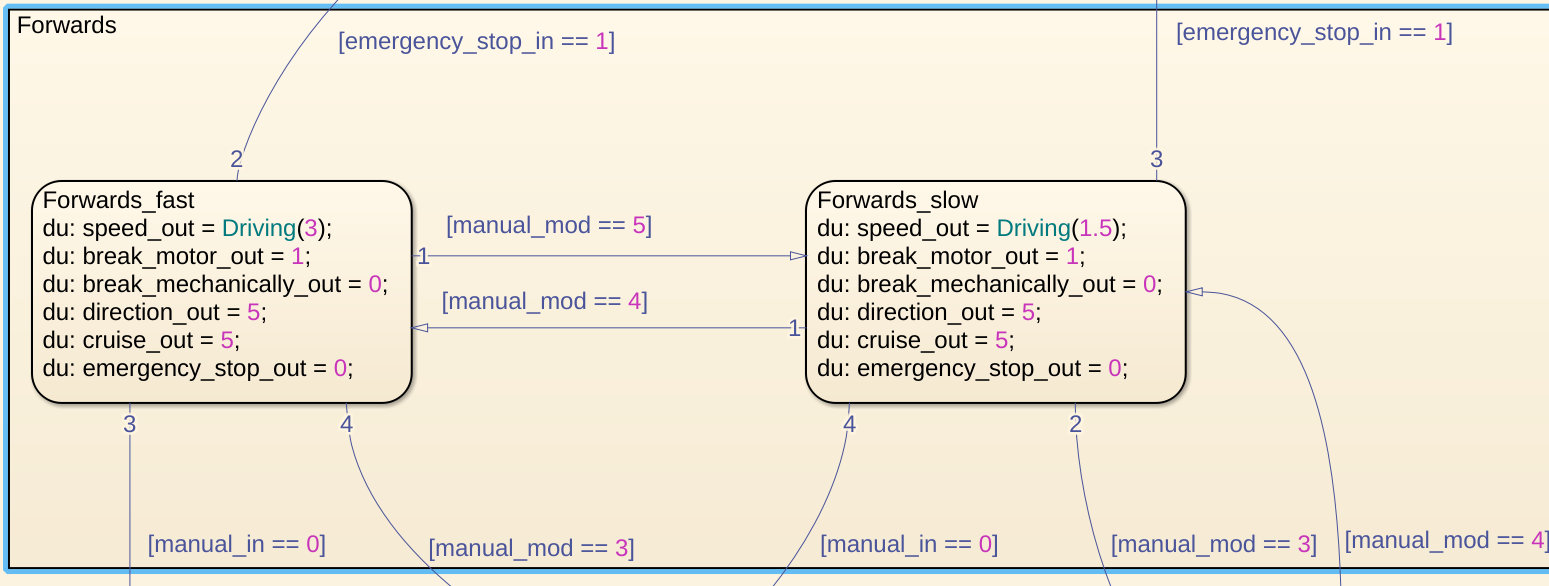
\includegraphics[width=\textwidth]{img/5_simulation/Automat_man_vorwaerts.png}
		\caption{Automat – vorwärts Stateflow der manuellen Steuerung}
		\label{Automat_man:img:man_vorwärts}
	\end{center}
\end{figure}
\pagebreak[1]



Mit dem Wahltaster (siehe Tabelle \ref{Controllpanel:tab:Wahlschalter}) kann zwischen den Zuständen gewechselt werden. In der Abbildung \ref{Automat_man:img:man_vorwärts} ist der Ausschnitt des vorwärts Stateflow zu sehen. Wenn sich der Automat in dem Stateflow vorwärts befindet, gibt es keine direkte verknüpfung zu dem rückwärts Stateflow, somit muss man erst in den Zustand \frqq Manuell Idle\flqq\ wechseln, um in den Stateflow rückwärts zu gelangen.

Der Zustand \frqq Sammler manuell in \flqq\ fängt  das Schaltsignal des Wahlschalters ab, wenn es mitten im Betrieb auf Automatik geschalten wird und führt zu dem \frqq Idle \flqq\ Zustand.









\subsubsection{Automat für die automatische Steuerung}
\label{Automatensteuerung:Automat_auto}

%\begin{center}
%
%	\begin{equation}
%		\label{Automat:equation:vektor_z_auto}
%		\vec{Z}_{A}= \left(\begin{array}{c} IDLE  \\ Drive \\ Distance \\ Stop \\ Emergency\ stop\end{array}\right)
%	\end{equation}
%
%	\begin{equation}
%		\label{Automat:equation:vektor_z_man}
%		\vec{Z}_{M}= \left(\begin{array}{c} IDLE  \\ Drive \\ Distance \\ Stop \\ Emergency\ stop\end{array}\right)
%	\end{equation}
%
%	\begin{equation}
%		\label{Automat:equation:vektor_i}
%		\vec{I}= \left(\begin{array}{c} speed_{in}  \\ distance_{in} \\ start_{in} \\ stop_{in} \\ reset_{in}\\ manual_{in} \\ manual_{mod}\\emergency\ stop_{in}  \end{array}\right)
%	\end{equation}
%
%	\begin{equation}
%		\label{Automat:equation:vektor_o}
%		\vec{O}= \left(\begin{array}{c} 1 \leqslant speed_{out} \leqslant 4 \\ break\ motor_{out} \in\ \{1,5\} \\ direction_{out} \in\ \{1,5\}\\ cruise_{out} \in\ \{1,5\} \\ break\ mechanically_{out}\in\ \{1,5\}  \end{array}\right)
%	\end{equation}\\ \ \\
%\end{center}




%Beim Ausgangsvektor \ref{Automat:equation:vektor_o} bedeutet der Wert 1, dass am Ausgang des  IO397-Moduls eine Spannung von 1 V anliegt, und bei einem Wert von 5 liegt am Ausgang eine Spannung von 5 V an. Der Ausgang $speed_{out}$ ist mit dem analogen Ausgang des IO397-Moduls verbunden, sodass die Spannung zwischen 1 V und 4 V variieren kann. Die Spannungsbereiche für die Eingänge des Vector-Controllers können zudem aus der Tabelle \ref{Vector_Controller:tab:pinmapping} entnommen werden.\\ \ \\


%Der Zustand $\mathbf{IDLE}$ ist der Startzustand des Fahrzeugs. In diesem Zustand wird die Motorbremse aktiviert, die Ausgangsgeschwindigkeit auf null gesetzt ($speed_{out} = 1$ entspricht logisch Null), die Funktion Driving aufgerufen und zurückgesetzt. Die Funktion Driving, siehe Abbildung \ref{Automat:img:fnc_Driving}, erhält einen Eingangswert, der durch einen \frqq Rate Limiter\flqq\  begrenzt und am Ausgang ausgegeben wird.
%Der Ausgang $direction_{out}$ ist



%\begin{equation}
%	\label{Automat:equation:vektor_o_1}
%	\vec{O}_{IDLE} = \left(\begin{array}{c} speed_{out} = 1 \\  break\ motor_{out} = 5\\ break\ mechanically_{out}= 0\\  direction_{out} = 5\\ cruise_{out} = 5 \end{array}\right)
%\end{equation}




\pagebreak[1]
\begin{figure}[!ht]
	\begin{center}
		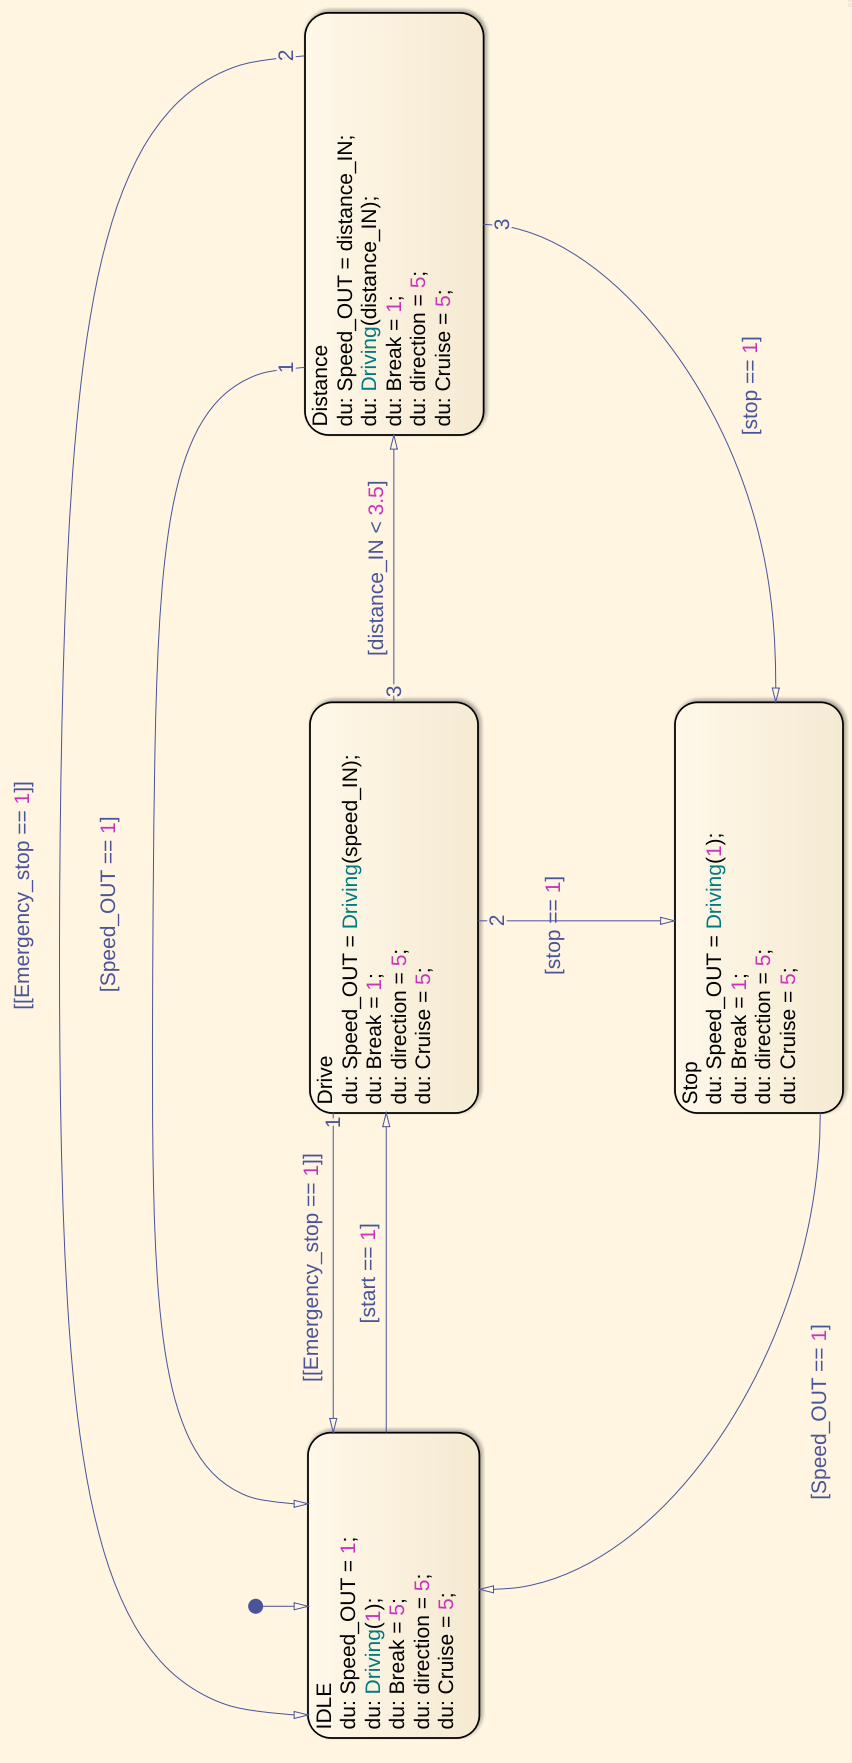
\includegraphics[height=0.86\textheight]{img/5_simulation/Automat_1.png}
		\caption{Simulation – Automat}
		\label{Automat:img:Automat}
	\end{center}
\end{figure}
\pagebreak[4]




%%%%%%%%%%%%%%%%%%%%%%%%%%%%%%%%%%%%%%%%%%%%%%%%%%%%%%%%%%%%%%%%%%%%%%%%%%%%%%%%%%%%
%%%%%%%%%%%%%%%%%%%%%%%%%%%%%%%%%%%%%%%%%%%%%%%%%%%%%%%%%%%%%%%%%%%%%%%%%%%%%%%%%%%%
%%%%%%%%%%%%%%%%%%%%%%%%%%%%%%%%%%%%%%%%%%%%%%%%%%%%%%%%%%%%%%%%%%%%%%%%%%%%%%%%%%%%
%%%%%%%%%%%%%%%%%%%%%%%%%%%%%%%%%%%%%%%%%%%%%%%%%%%%%%%%%%%%%%%%%%%%%%%%%%%%%%%%%%%%
%%%%%%%%%%%%%%%%%%%%%%%%%%%%%%%%%%%%%%%%%%%%%%%%%%%%%%%%%%%%%%%%%%%%%%%%%%%%%%%%%%%%
%%%%%%%%%%%%%%%%%%%%%%%%%%%%%%%%%%%%%%%%%%%%%%%%%%%%%%%%%%%%%%%%%%%%%%%%%%%%%%%%%%%%






\newpage
\section{Distanzmessung}

\myboxy{
	\begin{itemize}
		\item + Anschlüsse herauszufinden vier anschlüsse gefunden.
		\item + Was für Aufgaben haben die Anschlüsse?
		      \subitem Was für ein Kommunikationsprotokol hat der Sensor?
		      \subitem Asynchron und seriell mit Baudrate 115200. (Ozilloskop)
		\item mit einem ESP32 die Sensordaten lesen.
		\item Nachrichtdekodierung (Controller MCU)
		      \subitem Ox24 Start (Nachricht start)
		      \subitem 0x26 Stopp (Nachricht ende)
		      \subitem 24 30 30 30 33 32 36 30 30 32 39 26 (Stopp signal)
		      \subitem 24 30 30 30 33 32 36 30 31 33 30 26 (Laser an)
		      \subitem 24 30 30 30 32 32 31 32 33 26 (Messen)
	\end{itemize}}{To-do}{\textwidth}


Der Sensor von Pepperl+Fuchs wurde ursprünglich für die Distanzmessung angeschafft. Da dieser Sensor jedoch sehr teuer ist und wir nicht das Risiko eines möglichen Schadens im Vakuum eingehen wollten, wurde nach einer kostengünstigen Alternative gesucht.\\
Die Idee bestand darin, ein Entfernungsmessgerät von PARKSIDE zu verwenden und den Sensor aus dem Gerät zu entfernen. Die Messwerte werden anschließend mit einer MCU decodiert.

\subsection{Verbindung}
Der Sensor ist über ein Flachbandkabel mit der Hauptplatine verbunden, wie in Abbildung \ref{img_2_2:sen_dis_parkside:1} zu sehen ist. Auf der Hauptplatine befinden sich vier ungenutzte Lötstellen. Mithilfe eines Oszilloskops haben wir diese Lötstellen analysiert und festgestellt, dass Leitung eins eine Spannung von 3,3 V führt und Leitung vier als GND dient. Die Leitungen zwei und drei übertragen digitale Signale und fungieren als Datenleitungen.\\
Wenn zwei Leitungen für die Datenübertragung vorhanden sind, kann die Kommunikation bei einer zweiadrigen Verbindung entweder synchron oder asynchron erfolgen. Ist die Kommunikation synchron, dient eine der Leitungen als Taktleitung (Clock). Andernfalls, bei einer asynchronen Kommunikation, ist eine Leitung der Sender (TX) und die andere der Empfänger (RX). Dies ermöglicht eine Vollduplex-Übertragung.
Der Sensor komuniziert mit einem Bussystem.



\pagebreak[1]
\begin{figure}[ht]
	\begin{center}
		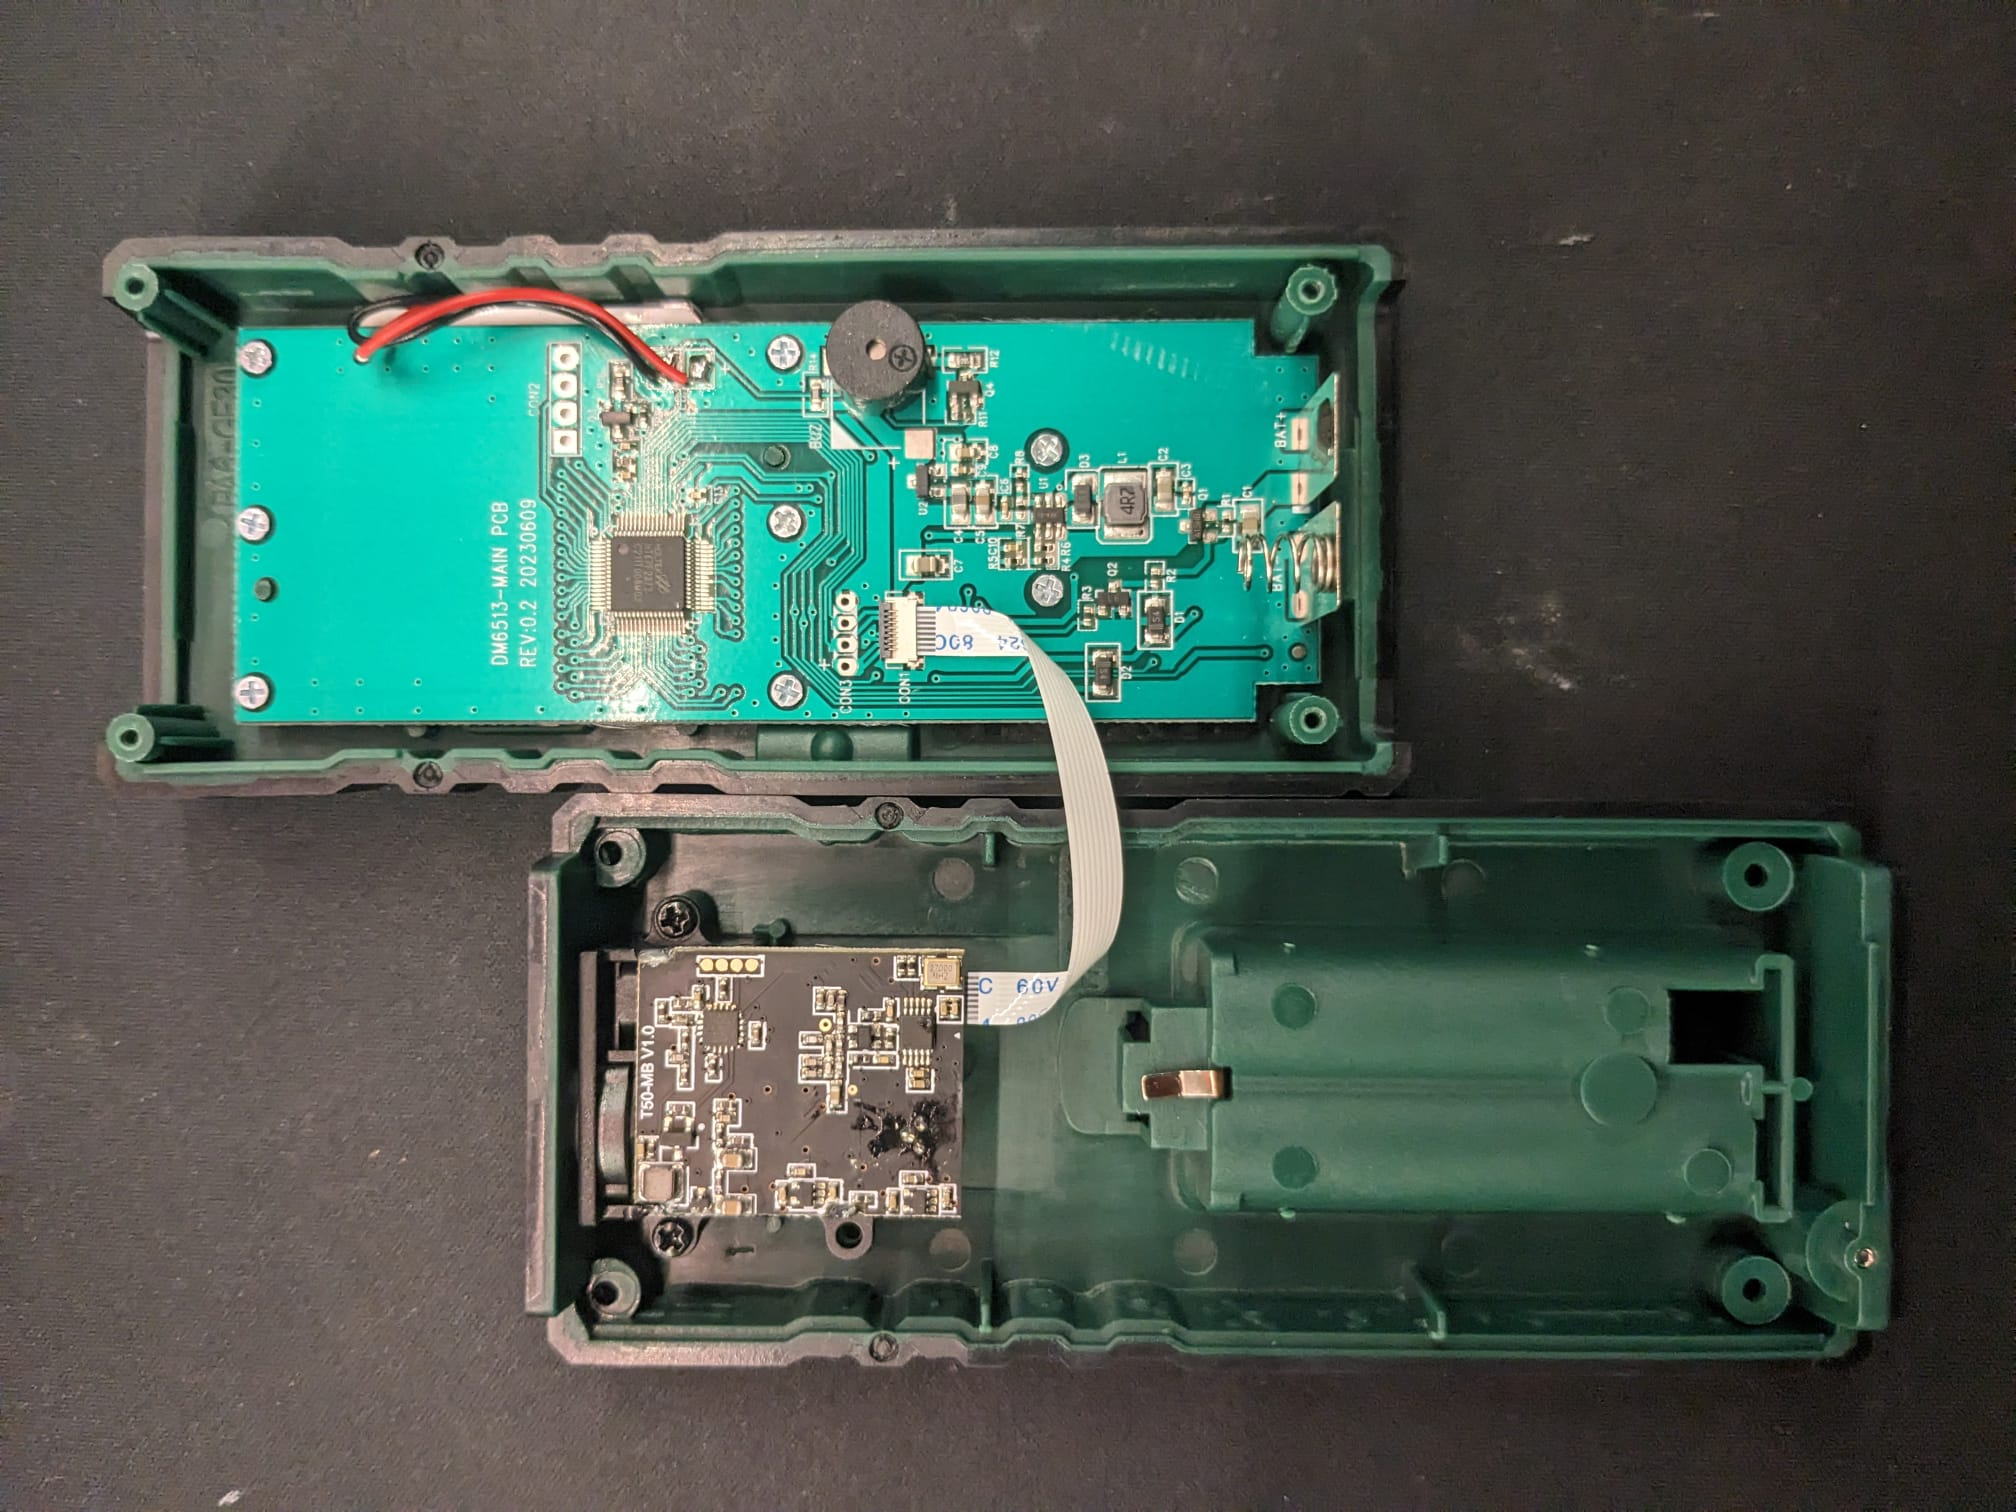
\includegraphics[width=1\textwidth]{img/2_sen/dis_parkside_1_outside.png}
		\caption{PARKSIDE – Distanzsensor – Innenaufbau}
		\label{img_2_2:sen_dis_parkside:1}
	\end{center}
\end{figure}
\pagebreak[1]

\pagebreak[1]
\begin{table}[ht]
	\centering
	\caption{PARKSIDE – Pin Mapping – Distanzsensor}
	\label{parkside:pinmapping}
	\begin{tabular}{l|ll}
		\hline
		\textbf{Pin} & \textbf{Farbe} & \textbf{Funktion} \\ \hline
		1            & Rot            & 3V3               \\
		2            & Weiß           & RX (receiver)     \\
		3            & Gelb           & TX (transmitter)  \\
		4            & Schwarz        & GND               \\ \hline
	\end{tabular}
\end{table}
\pagebreak[1]







%%%%%%%%%%%%%%%%%%%%%%%%%%%%%%%%%%%%%%%%%%%%%%%%%%%%%%%%%%%%%%%%%%%%%%%%%%%%%%%%%%%%
%%%%%%%%%%%%%%%%%%%%%%%%%%%%%%%%%%%%%%%%%%%%%%%%%%%%%%%%%%%%%%%%%%%%%%%%%%%%%%%%%%%%
%%%%%%%%%%%%%%%%%%%%%%%%%%%%%%%%%%%%%%%%%%%%%%%%%%%%%%%%%%%%%%%%%%%%%%%%%%%%%%%%%%%%
%%%%%%%%%%%%%%%%%%%%%%%%%%%%%%%%%%%%%%%%%%%%%%%%%%%%%%%%%%%%%%%%%%%%%%%%%%%%%%%%%%%%
%%%%%%%%%%%%%%%%%%%%%%%%%%%%%%%%%%%%%%%%%%%%%%%%%%%%%%%%%%%%%%%%%%%%%%%%%%%%%%%%%%%%
%%%%%%%%%%%%%%%%%%%%%%%%%%%%%%%%%%%%%%%%%%%%%%%%%%%%%%%%%%%%%%%%%%%%%%%%%%%%%%%%%%%%